\documentclass[letterpaper, 11pt]{article}
\usepackage[margin=1in]{geometry}

% Set the typeface to Times Roman
\usepackage{times}

%\usepackage{hyperref}
\usepackage{amsfonts}%
\usepackage{amssymb}%
\usepackage{amsthm}% allows theoremstyles (see below) and provides a proof environment
\usepackage{bm}
\usepackage{relsize}
\usepackage{graphicx}
\usepackage{caption}
\usepackage{epstopdf}
\usepackage{amsmath}
\usepackage{tikz}
\usetikzlibrary{trees,arrows}
\usetikzlibrary{decorations}
\usetikzlibrary[decorations]
\usepgflibrary{decorations.pathmorphing}
\usepgflibrary[decorations.pathmorphing]
\usetikzlibrary{decorations.pathmorphing}
\usetikzlibrary[decorations.pathmorphing]
\usepackage{booktabs}
\usepackage[authoryear]{natbib}
\usepackage{subcaption}
\usepackage{algorithm}
\usepackage[noend]{algpseudocode}
\usepackage{pseudocode}
%\usepackage{float}
\usepackage{verbatim} %% for commenting blocks
\usepackage[authoryear]{natbib}
\usepackage{url}

\bibpunct{(}{)}{,}{}{}{;} %% added this to make \citep{x} use parentheses

\newcommand{\problemAnswer}[1]{%#1% Defines the problem answer command with the content as the only argument
\noindent\framebox[0.95\columnwidth][c]{\begin{minipage}{0.92\columnwidth}\color{blue}{#1}\end{minipage}} % Makes the box around the problem answer and puts the content inside
}

%% independence symbol and expectation operator %%
\newcommand\independent{\protect\mathpalette{\protect\independenT}{\perp}}
\def\independenT#1#2{\mathrel{\rlap{$#1#2$}\mkern2mu{#1#2}}}

\DeclareMathOperator{\circlearrow}{\hbox{$\circ$}\kern-1.5pt\hbox{$\rightarrow$}}
\DeclareMathOperator{\circlecircle}{\hbox{$\circ$}\kern-1.2pt\hbox{$--$}\kern-1.5pt\hbox{$\circ$}}

\DeclareMathOperator{\an}{an}
\DeclareMathOperator{\pa}{pa}
\DeclareMathOperator{\ch}{ch}
\DeclareMathOperator{\pre}{pre}
\DeclareMathOperator{\de}{de}
\DeclareMathOperator{\nd}{nd}
\DeclareMathOperator{\sib}{sib}
\DeclareMathOperator{\dis}{dis}
\DeclareMathOperator{\mb}{mb}
\DeclareMathOperator{\omb}{omb}
\DeclareMathOperator{\doo}{do}
\DeclareMathOperator{\odds}{\text{OR}}
\DeclareMathOperator*{\argmax}{arg\,max}
\DeclareMathOperator*{\argmin}{arg\,min}
\definecolor{lemon}{RGB}{ 242, 200,  24}
\def\ci{\perp\!\!\!\perp}
\newcommand{\E}{\mathbb{E}}
\newcommand{\G}{\mathcal{G}}

\newcommand\indep{\protect\mathpalette{\protect\independenT}{\perp}}
\def\independenT#1#2{\mathrel{\rlap{$#1#2$}\mkern2mu{#1#2}}}

\newtheorem{Lma}{Lemma}
\newtheorem{Thm}{Theorem}

\DeclareMathOperator{\diedgeright}{\textcolor{blue}{\boldsymbol{\rightarrow}}}
\DeclareMathOperator{\diedgeleft}{\textcolor{blue}{\boldsymbol{\leftarrow}}}
\DeclareMathOperator{\biedge}{\textcolor{red}{\boldsymbol{\leftrightarrow}}}
\DeclareMathOperator{\udedge}{\textcolor{brown}{\boldsymbol{\textendash}}}
%%%%%%%%%%%%%%%%%%%%%%%%%%%%

\title{CS 476/676 (Spring 2021): Homework 4}

\author{}

\date{Due: Mar 17, 2021 at 11:59pm EST}

\begin{document}

\maketitle

\setlength{\parindent}{0em}
\setlength{\parskip}{0.8em}

\large\textbf{Name:} \underline{\hspace{30pt} \color{blue} Josh Popp \hspace{30pt}}
\vspace{1em}

	\textbf{Instructions}: This homework requires answering some open-ended questions, proofs, and analysis. This is an individual assignment, not group work. Though you may discuss the problems with your classmates, you must solve the problems and write the solutions independently. As stated in the syllabus, copying code
	from a classmate or the internet (even with minor changes) constitutes plagiarism. You are required to submit your answers in pdf form (use \LaTeX) in a file called \texttt{<your-JHED>-hw4.pdf} to Gradescope under ``HW4''.
	Late submissions will be penalized, except in extenuating circumstances such
	as medical or family emergency. Submissions submitted 0-24 hours late will be
	penalized 10\%, 24-48 hours late by 20\%, 48-72 hours late by 30\%, and later
    than 72 hours by 100\%. Late days may be used (if available) to avoid these penalties.

    The total assignment is worth 90 points.

    \textbf{Important note:} For  portions of the assignment that require drawing graphs, we  encourage you to use the \LaTeX\  template provided to draw graphs using the \texttt{tikz} package. However, hand drawing graphs/using other software and then including the images into the pdf using \texttt{includegraphics} is also acceptable as long as it is neat.



\vspace{2em}

{\large\textbf{Problem 1}} (10 points)

Recall our motivation for using an ADMG $\G(V)$ to summarize the joint distribution on observed variables $V$ in a latent variable DAG $\G(V \cup U)$ was to preserve all \textbf{causal} and \textbf{statistical} information on the observed variables $V$ without explicitly thinking about the latent variables $U$. Refer to the lecture slides for precise definitions of what is meant by preserving all causal and statistical information.

Imagine the second rule of the latent projection operator was modified to read as follows:

$V_i \biedge V_j$ exists in $\G(V)$ if there exists a path $V_i \diedgeleft \cdots \diedgeright V_j$ in $\G(V \cup U)$ such that all intermediate vertices are unmeasured variables in $U.$

That is, we do not have the additional check that there are no colliders along such paths. Answer the following questions.

1) Prove, via a suitable counterexample of a latent variable DAG and the ADMG obtained using the modified latent projection operator, that the absence of this additional check results in ADMGs that do not correctly preserve statistical information among the observed variables. (5 points)

\problemAnswer{

Latent variable DAG
$$ V_1 \diedgeleft U_1 \diedgeright U_2 \diedgeleft U_3 \diedgeright V_2 $$
Proposed ADMG
$$ V_1 \biedge V_2 $$
Under the latent variable DAG, $ V_1 \ci V_2 $, but under the proposed ADMG, this conditional independence does not hold because we failed to account for the collider along the path from $V_1$ to $V_2$ when determining whether to place a bidirected edge between the two nodes.
}

2) Does the absence of the additional check also affect the preservation of causal information in the ADMG $\G(V)$? Why or why not? (5 points)

\problemAnswer{
Yes, this does also affect the preservation of causal information. The latent variable DAG suggests distinct unobserved causes for $V_1$ and $V_2$ (and has no open path from $V_1$ to $V_2$ since we don't observe the collider $U_2$), while the proposed ADMG suggests a common unobserved cause for the two variables (and has an open bidirected path $V_1 \biedge V_2$).
}
\vspace{1em}

Remember to rely on the precise formal definitions as stated in the lecture slides of what we mean by preserving causal and statistical information when answering 1) and 2).

\vspace{1em}

{\large\textbf{Problem 2}} (10 points)

Please ask any questions regarding Problem 2 (so only for this problem) via \textbf{private} Piazza posts, as it is easy to accidentally give away the solution to this problem.

Draw all ADMGs that are Markov equivalent (that is, imply the exact same m-separation relations) to,

1) the ADMG shown in Figure~\ref{fig:prob2}a (5 points) \\
2) the ADMG shown in Figure~\ref{fig:prob2}b (5 points)

\begin{figure}[h]
	\begin{center}
		\scalebox{1}{
			\begin{tikzpicture}[>=stealth, node distance=1.5cm]
			\tikzstyle{format} = [draw, thick, circle, minimum size=1.0mm, inner sep=0pt]
			\tikzstyle{square} = [draw, thick, minimum size=1.0mm, inner sep=3pt]

			\begin{scope}
			\path[->, very thick]

			node[] (a) {$A$}
			node[right of=a] (b) {$B$}
			node[right of=b] (c) {$C$}
			node[below right of=a, xshift=0.5cm] {(a)}

			(a) edge[red, <->] (b)
			(b) edge[red, <->] (c)
			;
			\end{scope}

			\begin{scope}[xshift=6cm, yshift=1cm]
			\path[->, very thick]

			node[] (a) {$A$}
			node[right of=a] (b) {$B$}
			node[below of=a] (c) {$C$}
			node[below of=b] (d) {$D$}
			node[below right of=c, xshift=-0.25cm] {(b)}

			(a) edge[red, <->] (b)
			(b) edge[red, <->] (d)
			(c) edge[red, <->] (d)
			(a) edge[red, <->] (c)
			;
			\end{scope}

			\end{tikzpicture}
		}
	\end{center}
	\caption{}
	\label{fig:prob2}
\end{figure}

\problemAnswer{
For the first one, constraining to bow-free ADMGs, the following are all Markov equivalent
\begin{center}
	\scalebox{1}{
		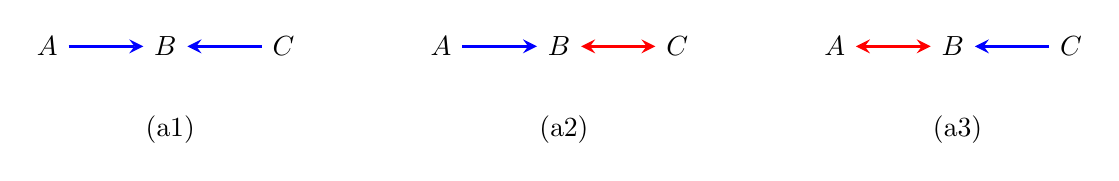
\begin{tikzpicture}[>=stealth, node distance=1.5cm]
		\tikzstyle{format} = [draw, thick, circle, minimum size=1.0mm, inner sep=0pt]
		\tikzstyle{square} = [draw, thick, minimum size=1.0mm, inner sep=3pt]

		\begin{scope}
		\path[->, very thick]

		node[] (a) {$A$}
		node[right of=a] (b) {$B$}
		node[right of=b] (c) {$C$}
		node[below right of=a, xshift=0.5cm] {(a1)}

		(a) edge[blue, ->] (b)
		(b) edge[blue, <-] (c)
		;
		\end{scope}

		\begin{scope}[xshift=5cm]
		\path[->, very thick]

		node[] (a) {$A$}
		node[right of=a] (b) {$B$}
		node[right of=b] (c) {$C$}
		node[below right of=a, xshift=0.5cm] {(a2)}

		(a) edge[blue, ->] (b)
		(b) edge[red, <->] (c)
		;
		\end{scope}

		\begin{scope}[xshift=10cm]
		\path[->, very thick]

		node[] (a) {$A$}
		node[right of=a] (b) {$B$}
		node[right of=b] (c) {$C$}
		node[below right of=a, xshift=0.5cm] {(a3)}

		(a) edge[red, <->] (b)
		(b) edge[blue, <-] (c)
		;
		\end{scope}

		\end{tikzpicture}
	}
\end{center}
If we're expanding beyond bow-free ADMGs, any bidirected edge (in any of these four graphs) can be accompanied by a directed edge pointing towards $B$. For the second one, there are no bow-free Markov equivalent ADMGs.
\begin{center}
	\scalebox{1}{
		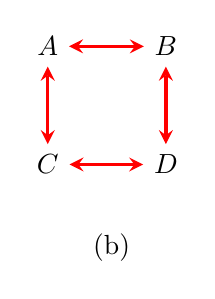
\begin{tikzpicture}[>=stealth, node distance=1.5cm]
		\tikzstyle{format} = [draw, thick, circle, minimum size=1.0mm, inner sep=0pt]
		\tikzstyle{square} = [draw, thick, minimum size=1.0mm, inner sep=3pt]

		\begin{scope}[]
		\path[->, very thick]

		node[] (a) {$A$}
		node[right of=a] (b) {$B$}
		node[below of=a] (c) {$C$}
		node[below of=b] (d) {$D$}
		node[below right of=c, xshift=-0.25cm] {(b)}

		(a) edge[red, <->] (b)
		(b) edge[red, <->] (d)
		(c) edge[red, <->] (d)
		(a) edge[red, <->] (c)
		;
		\end{scope}

		\end{tikzpicture}
	}
\end{center}
Directed edges can be added in any way that avoids a directed path of length greater than 1 (ie, $\circ \diedgeright \circ \diedgeright \circ$ is not allowed)
}

\vspace{1em}

{\large\textbf{Problem 3}} (10 points)

\begin{figure}[h]
	\begin{center}
		\scalebox{1}{
			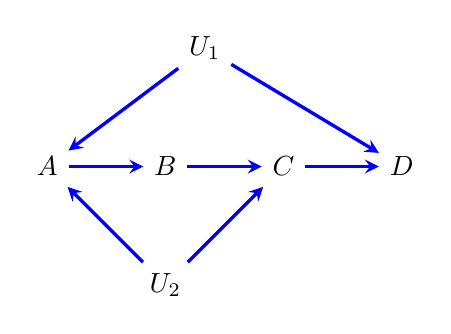
\begin{tikzpicture}[>=stealth, node distance=1.5cm]
			\tikzstyle{format} = [draw, thick, circle, minimum size=1.0mm, inner sep=0pt]
			\tikzstyle{square} = [draw, thick, minimum size=1.0mm, inner sep=3pt]
			\begin{scope}
			\path[->, very thick]

			node[] (a) {$A$}
			node[right of=a] (b) {$B$}
			node[right of=b] (c) {$C$}
			node[right of=c] (d) {$D$}
			node[above of=b, xshift=0.5cm] (u1) {$U_1$}
			node[below of=b] (u2) {$U_2$}

			(a) edge[blue] (b)
			(b) edge[blue] (c)
			(c) edge[blue] (d)
			(u1) edge[blue] (a)
			(u1) edge[blue] (d)
			(u2) edge[blue] (a)
			(u2) edge[blue] (c)
			;
			\end{scope}

			\end{tikzpicture}
		}
	\end{center}
	\caption{}
	\label{fig:prob3}
\end{figure}

Consider the latent variable DAG shown in Figure~\ref{fig:prob3} where $U_1$ and $U_2$ are unmeasured/latent. Prove, using the proof technique shown in Lecture 9 for deriving generalized equality constraints, that the kernel defined below is not a function of $B$.

\begin{align*}
q_D(D \mid A, B, C) \equiv \frac{\sum_A p(A)\times p(C, D \mid A, B)}{\sum_A p(A)\times p(C\mid A, B)}
\end{align*}

\vspace{1em}

\problemAnswer{
\begin{align*}
\sum_A p(A)\times p(C, D \mid A, B) &= \sum_A p(A) \sum_{U_1}p(C,D,U_1 \mid A, B) \\
&= \sum_A p(A) \sum_{U_1}p(D,U_1 \mid A, B, C) p(C \mid A, B) \\
&= \sum_A p(A) \sum_{U_1}p(D \mid A, B, C, U_1 )  p(U_1 \mid A, B, C) p(C \mid A, B) \\
&= \sum_A p(A) p(C \mid A, B) \sum_{U_1}p(D \mid C, U_1 )  p(U_1 \mid A,B,C) \\
&= \sum_A p(A) p(C \mid A, B) \sum_{U_1}p(D \mid C, U_1 )  \sum_{U_2}p(U_1 , U_2 \mid A,B,C) \\
&= \sum_A p(A) p(C \mid A, B) \sum_{U_1}p(D \mid C, U_1 )  \sum_{U_2}p(U_1 \mid A,B,C, U_2) \\ &\times p(U_2 \mid A,B,C) \\
&= \sum_A p(A) p(C \mid A, B) \sum_{U_1}p(D \mid C, U_1 )  \sum_{U_2}p(U_1 \mid A,U_2) \\ &\times p(U_2 \mid A,B,C) \\
&= \sum_{U_1}p(D \mid C, U_1 ) \\ &\times \sum_A p(A) p(C \mid A, B)   \sum_{U_2}p(U_1 \mid A,U_2) p(U_2 \mid A,B,C)
\end{align*}
}
\vspace{1em}

{\large\textbf{Problem 4}} (20 points)

\begin{figure}[h]
	\begin{center}
		\scalebox{1}{
			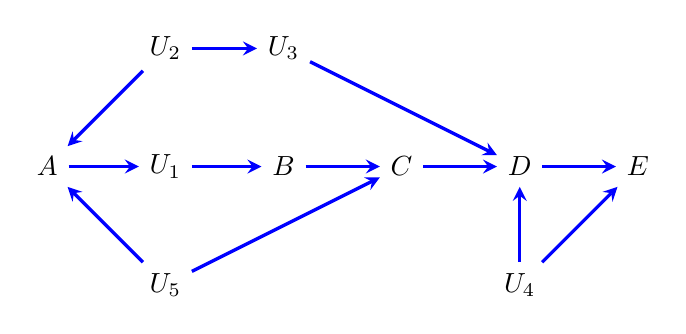
\begin{tikzpicture}[>=stealth, node distance=1.5cm]
			\tikzstyle{format} = [draw, thick, circle, minimum size=1.0mm, inner sep=0pt]
			\tikzstyle{square} = [draw, thick, minimum size=1.0mm, inner sep=3pt]
			\begin{scope}
			\path[->, very thick]

			node[] (a) {$A$}
			node[right of=a] (u1) {$U_1$}
			node[right of=u1] (b) {$B$}
			node[right of=b] (c) {$C$}
			node[right of=c] (d) {$D$}
			node[right of=d] (e) {$E$}
			node[above of=u1] (u2) {$U_2$}
			node[right of=u2] (u3) {$U_3$}
			node[below of=d] (u4) {$U_4$}
			node[below of=u1] (u5) {$U_5$}

			(a) edge[blue] (u1)
			(u1) edge[blue] (b)
			(b) edge[blue] (c)
			(c) edge[blue] (d)
			(d) edge[blue] (e)
			(u2) edge[blue] (a)
			(u2) edge[blue] (u3)
			(u3) edge[blue,] (d)
			(u4) edge[blue] (d)
			(u4) edge[blue] (e)
			(u5) edge[blue] (a)
			(u5) edge[blue] (c)
			;
			\end{scope}

			\end{tikzpicture}
		}
	\end{center}
	\caption{}
	\label{fig:prob4}
\end{figure}

Consider the latent variable DAG in Figure~\ref{fig:prob4} where $U_1, U_2, U_3, U_4, U_5$ are latent.

1) Draw the latent variable ADMG $\G(V)$ on the observed variables $V = \{A, B, C, D, E\}$. (5 points)

\problemAnswer{
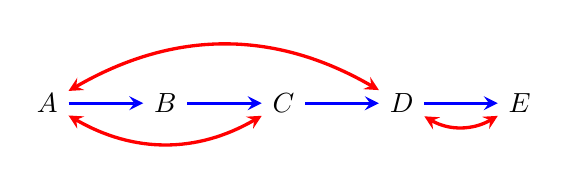
\begin{tikzpicture}[>=stealth, node distance=1.5cm]
			\tikzstyle{format} = [draw, thick, circle, minimum size=1.0mm, inner sep=0pt]
			\tikzstyle{square} = [draw, thick, minimum size=1.0mm, inner sep=3pt]
			\begin{scope}
			\path[->, very thick]

			node[] (a) {$A$}
			node[right of=a] (b) {$B$}
			node[right of=b] (c) {$C$}
			node[right of=c] (d) {$D$}
			node[right of=d] (e) {$E$}

			(a) edge[blue] (b)
			(b) edge[blue] (c)
			(c) edge[blue] (d)
			(d) edge[blue] (e)

			(a) edge[red, <->, out=330, in=210] (c)
			(a) edge[red, <->, out=30, in=150] (d)
			(d) edge[red, <->, out=330, in=210] (e)
			;
			\end{scope}

			\end{tikzpicture}
}
\vspace{1em}

2) Apply m-separation to the latent variable ADMG $\G(V)$ from part 1) to answer the following questions. Justify each of your answers, i.e., list at least one open path if there is one. Is, (3 points each) \\[0.5em]
a) $C\ci E \mid D?$ \\
b) $B\ci D \mid A, C?$ \\
b) $B\ci E \mid A, C, D?$

\problemAnswer{
a) No, $D$ is a collider, opening the path $$ C \diedgeright D \biedge E$$
b) No, since $A$ and $C$ are both colliders we open up a path from $B$ to $D$ by conditioning on them
$$B \diedgeright C \biedge A \biedge D $$
\\
c) No, once again, $C$, $A$, and $D$ are colliders so we open up $$B \diedgeright C \biedge A \biedge D \biedge E$$
}
\vspace{1em}

3) Find and describe, using the algorithm provided in Lecture 11, a Verma constraint implied by the ADMG $\G(V)$ from part 1). If you are unable to find a constraint, this might be an indication that you did not derive the ADMG $\G(V)$ in part 1) correctly, or you may not be applying the algorithm correctly. That is, there exists at least one Verma constraint in the correct latent projection ADMG. (6 points)

\vspace{1em}
\problemAnswer{
1. There is an inducing path from $A$ to $E$, $A \biedge D \diedgeright E$ \\
2. $B$ is fixable, since it has no bidirected edges. Fixing it breaks the inducing path by removing the direct edge from $A$ to $B$, such that $E$ is no longer a descendant of $A$. \\
3. (In the slides, this is an extra step for when our fixable vertex is one of the endpoints of the inducing path, which it's not here) \\
4. Since $\omb{(B)}= \{ A \}$, we take $q=p(V)/p(B \mid A)$ and $\G^q$ is the following graph
\begin{center}
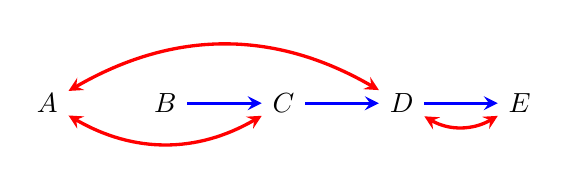
\begin{tikzpicture}[>=stealth, node distance=1.5cm]
			\tikzstyle{format} = [draw, thick, circle, minimum size=1.0mm, inner sep=0pt]
			\tikzstyle{square} = [draw, thick, minimum size=1.0mm, inner sep=3pt]
			\begin{scope}
			\path[->, very thick]

			node[] (a) {$A$}
			node[right of=a] (b) {$B$}
			node[right of=b] (c) {$C$}
			node[right of=c] (d) {$D$}
			node[right of=d] (e) {$E$}

			(b) edge[blue] (c)
			(c) edge[blue] (d)
			(d) edge[blue] (e)

			(a) edge[red, <->, out=330, in=210] (c)
			(a) edge[red, <->, out=30, in=150] (d)
			(d) edge[red, <->, out=330, in=210] (e)
			;
			\end{scope}

			\end{tikzpicture}
			\end{center}
So we have the Verma constraint $A \ci_q E$
}
\vspace{1em}

{\large\textbf{Problem 5}} (15 points)

A mixed graph $\G$ on $d$ variables $V_1, \dots, V_d$ consisting of directed ($\diedgeright$) and bidirected ($\biedge$) edges can be summarized via two binary adjacency matrices $D$ and $B$ as follows.

$D_{ij} = 1$ if $V_i \diedgeright V_j$ exists in $\G$ and $D_{ij} = 0$ otherwise.\\
$B_{ij}=B_{ji} = 1$ if $V_i \biedge V_j$ exists in $\G$ and $B_{ij} = B_{ji} = 0$ otherwise.

Recall in HW3 you proved that $\G$ is acyclic (contains no directed cycles) if and only if $\text{trace}(e^D) - d = 0$. That is, $\G$ is an acyclic directed mixed graph (ADMG) if and only if  $\text{trace}(e^D) - d = 0$. Often, we also want to impose certain requirements on the way bidirected edges appear in $\G$. This is because when there are no restrictions imposed, $\G$ is not a simple graph (could have more than one edge between each pair of vertices), which complicates statistical inference in the underlying models.\footnote{In the sense that the corresponding model may not be identified from observed data. That is, its parameters cannot be computed in an unbiased fashion. We will formalize what this means in class, but it is tangential to solving Problem 5.}

\textbf{Important note:} For simplicity, in the following proofs you may assume that the diagonal elements of $D$ and $B$ are always $0$, i.e., ``self edges'' of the form $V_i \diedgeright V_i$ and $V_i \biedge V_i$ are ruled out apriori.

a) One popular subclass of ADMGs, is the class of bow-free ADMGs. Besides acyclicity, bow-free ADMGs have the additional restriction that for any pair of vertices $V_i, V_j$, both $V_i \diedgeright V_j$ and $V_i \biedge V_j$ do not appear in $\G$.\footnote{The term bow-free comes from the fact that when both  $V_i \diedgeright V_j$ and $V_i \biedge V_j$ are present, the edges often look like a bow ready to shoot (in the archery sense) -- you can refer to the lecture slides to see what I mean.} That is, bow-free ADMGs form the class of all simple ADMGs. Prove that an ADMG $\G$ is bow-free if and only if $\text{sum}(D \circ B) = 0,$ where $X \circ Y$ denotes the elementwise matrix product a.k.a Hadamard product of $X$ and $Y,$ and $\text{sum}(X)$ represents taking the sum of all elements of the matrix $X$. (4 points)

\problemAnswer{
Since $D_{ij} \in \{ 0, 1 \}$ and $B_{ij} \in \{ 0, 1 \} \ \forall \{ i, j \}$, $D_{ij} * B_{ij} \in \{ 0, 1 \}\ \forall \{ i, j \}$. Then $\text{sum}({D \circ B}) = \sum_{i,j} D_{ij} * B_{ij}=0$ IFF $\nexists \{k,l\} \text{ s.t. } D_{kl} = B_{kl} = 1$. $D_{kl} = B_{kl} = 1$ specifically corresponds to the condition of having a bow between $V_k$ and $V_l$ in $\G$ (both $V_k \diedgeright V_l$ and $V_k \biedge V_l$), so $\G$ is bow-free IFF $\text{sum}({D \circ B}) = 0$
}
\vspace{1em}

b) Another popular subclass of ADMGs, is the class of ancestral ADMGs. Besides acyclicity, ancestral ADMGs have the additional restriction that for any pair of vertices $V_i, V_j$, both a directed path $V_i \diedgeright \cdots \diedgeright V_j$ and $V_i \biedge V_j$ do not appear in $\G$. In other words, for every $V_i$ it is the case that $\an_\G(V_i) \cap \sib_\G(V_i) = \emptyset$.  Given the elementary operations we have used so far in proving various constraints on graphical structures -- the matrix exponential $e^D$ and its relation to directed paths in $\G$ (see HW3, Problem 4.1), the elementwise matrix product $X \circ Y$ between two matrices $X$ and $Y$, and the operation $\text{sum}(X)$ where we sum up all elements of a matrix $X$ -- design a function $f(D, B)$ based on these operations that is zero if and only if $\G$ is ancestral. That is, design and prove your function $f(D, B) = 0$ if and only if $\G$ is ancestral. (11 points)

\vspace{1em}
\problemAnswer{
$$f(D,B)=\text{sum}(e^D \circ B)=0 \text{ iff } \G \text { ancestral}$$
\emph{Proof}: $\text{sum}(e^D \circ B)=0 \text{ iff } \nexists \{ k,l \} \text{ s.t. } (e^D_{kl} \neq 0) \cap (B_{kl} \neq 0)$. So we want to show that $\nexists \{ k,l \} \text{ s.t. } (e^D_{kl} \neq 0) \cap (B_{kl} \neq 0) \text{ iff } \G \text{ ancestral}$. \\ \\
1. $\G \text{ ancestral} \implies \nexists \{ k,l \} \text{ s.t. } (e^D_{kl} \neq 0) \cap (B_{kl} \neq 0)$ \\ \\
$e_{kl}^D$ is a normalized count of the total number of paths $V_k \diedgeright ... \diedgeright V_l$, of any length, in $\G$. Since $\G$ is ancestral, for any vertices between which a path $V_k \diedgeright ... \diedgeright V_l$ (of length greater than or equal to 1) exists ($\implies e^D_{kl} \neq 0$), we know there's no bidirected edge $V_k \biedge V_l$ allowed ($\implies B_{kl}=0$), and vice versa ($B_{kl} \neq 0 \implies e^D_{kl} = 0$). A path of length zero can only exist from $V_k$ to $V_k$ (and does exist for all $k$), but we imposed an a priori constraint that $B_{kk}=0$ for all $k$. \\ \\
2. $\neg \G \text{ ancestral} \implies \exists \{ k,l \} \text{ s.t. } (e^D_{kl} \neq 0) \cap (B_{kl} \neq 0)$ \\ \\
If $\G$ is not ancestral, there exists some pair of nodes $V_k$ and $V_l$, $k \neq l$ such that $V_k \diedgeright ... \diedgeright V_l$ and $V_k \biedge V_l$ both exist in $\G$. Then $e^D_{kl} > 0$ since this is a normalized count of such paths in $D$, and $B_{kl}=1$ by the definition of the matrix $B$. \\ \\
Together, these prove that $\G \text{ ancestral} \iff \nexists \{ k,l \} \text{ s.t. } (e^D_{kl} \neq 0) \cap (B_{kl} \neq 0) \iff \text{sum}(e^D \circ B)=0 $
}

\vspace{1em}


{\large\textbf{Problem 6}} (25 points)

\begin{figure}
	\centering
	\begin{subfigure}{.5\textwidth}
		\centering
		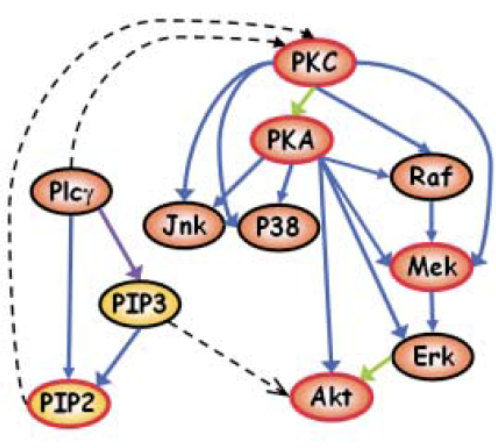
\includegraphics[width=.6\linewidth]{sachs_network}
		\vspace{3em}
%		\caption{The DAG learned by \cite{sachs2005causal}}
		\caption{}
		\label{fig:prob6a}
	\end{subfigure}%
	\begin{subfigure}{.5\textwidth}
		\centering
		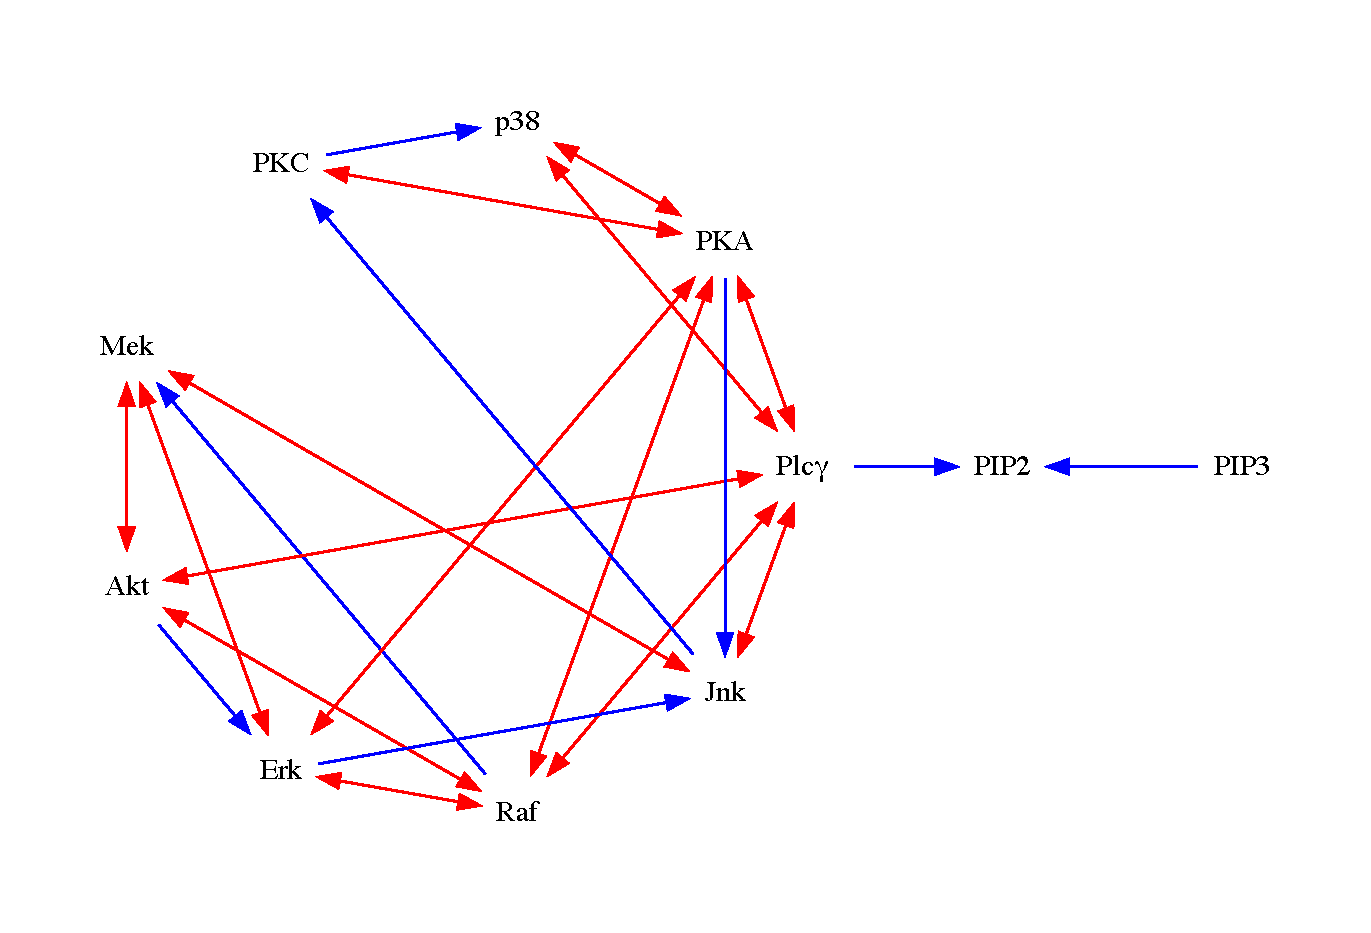
\includegraphics[width=1\linewidth]{sachs_admg}
		\caption{}
%		\caption{An ADMG learned for the protein/lipid expression data}
		\label{fig:prob6b}
	\end{subfigure}
	\caption{}
	\label{fig:prob6}
\end{figure}

\vspace{1em}

\begin{figure}[t]
	\begin{center}
		\scalebox{0.85}{
			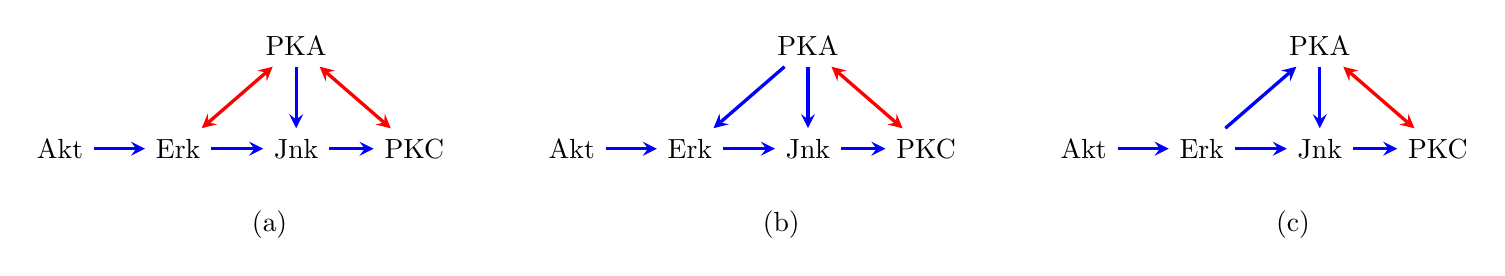
\begin{tikzpicture}[>=stealth, node distance=1.5cm]
			\tikzstyle{format} = [thick, circle, minimum size=1.0mm, inner sep=0pt]
			\tikzstyle{square} = [draw, thick, minimum size=1.0mm, inner sep=3pt]

			\begin{scope}[xshift=0cm]
			\path[->, very thick]
			node[] (akt) {Akt}
			node[right of=akt] (erk) {Erk}
			node[right of=erk] (jnk) {Jnk}
			node[right of=jnk] (pkc) {PKC}
			node[above of=jnk, yshift=-0.2cm] (pka) {PKA}
			node[below right of=erk, xshift=0.1cm, yshift=0.1cm] (label) {(a)}

			(akt) edge[blue] (erk)
			(erk) edge[blue] (jnk)
			(jnk) edge[blue] (pkc)
			(pka) edge[blue] (jnk)
			(erk) edge[red, <->] (pka)
			(pka) edge[red, <->] (pkc)
			;
			\end{scope}

			\begin{scope}[xshift=6.5cm]
			\path[->, very thick]
			node[] (akt) {Akt}
			node[right of=akt] (erk) {Erk}
			node[right of=erk] (jnk) {Jnk}
			node[right of=jnk] (pkc) {PKC}
			node[above of=jnk, yshift=-0.2cm] (pka) {PKA}
			node[below right of=erk, xshift=0.1cm, yshift=0.1cm] (label) {(b)}

			(akt) edge[blue] (erk)
			(erk) edge[blue] (jnk)
			(jnk) edge[blue] (pkc)
			(pka) edge[blue] (jnk)
			(pka) edge[blue] (erk)
			(pka) edge[red, <->] (pkc)
			;
			\end{scope}

			\begin{scope}[xshift=13cm]
			\path[->, very thick]
			node[] (akt) {Akt}
			node[right of=akt] (erk) {Erk}
			node[right of=erk] (jnk) {Jnk}
			node[right of=jnk] (pkc) {PKC}
			node[above of=jnk, yshift=-0.2cm] (pka) {PKA}
			node[below right of=erk, xshift=0.1cm, yshift=0.1cm] (label) {(c)}

			(akt) edge[blue] (erk)
			(erk) edge[blue] (jnk)
			(jnk) edge[blue] (pkc)
			(pka) edge[blue] (jnk)
			(erk) edge[blue] (pka)
			(pka) edge[red, <->] (pkc)
			;
			\end{scope}

			\end{tikzpicture}
		}
	\end{center}
	\caption{(a) A subgraph of the protein network in Figure~\ref{fig:prob6b}}
	\label{fig:supp_protein}
\end{figure}

In the last homework you learned how you might design a greedy causal discovery procedure to learn a DAG from data. If you suspect that there are unobserved variables in the problem, you may design a similar  procedure to learn an ADMG from data using the constraints you have derived in Problem 5. The output of such a procedure when applied to the same data from HW4, i.e., from the paper by \cite{sachs2005causal}, is displayed in Figure~\ref{fig:prob6b}.\footnote{We will learn the formal details of such procedures in the coming weeks, but they are not important for this problem.} The DAG learned by the original authors is displayed in Figure~\ref{fig:prob6a}.

As you can see, the ADMG in Figure~\ref{fig:prob6b} posits that there may exist many relations that arise due to unmeasured confounding rather than causation -- this possibility was also acknowledged by the authors of \cite{sachs2005causal}. Some of these bidirected edges miss the mark, e.g., Figure~\ref{fig:prob6b} has $\text{Raf} \diedgeright \text{Mek} \biedge \text{Erk}$ rather than $\text{Raf} \diedgeright \text{Mek} \diedgeright \text{Erk}$, but others present interesting alternatives to the hypotheses suggested by \cite{sachs2005causal}. We will study one of these in this problem.

In Figure~\ref{fig:prob6a}, there is an edge $\text{PKA} \diedgeright \text{Erk}$. The authors of \cite{sachs2005causal} performed an experiment where they manipulated expression of Erk to confirm that this has no downstream effect on PKA, and took this as evidence for the edge $\text{PKA} \diedgeright \text{Erk}$. However, in the absence of an experiment to show that manipulation of PKA does indeed cause downstream change in Erk, we cannot be sure if the association between them is due to causation ($\text{PKA} \diedgeright \text{Erk}$) as suggested by Figure~\ref{fig:prob6a} or unmeasured confounding ($\text{PKA} \biedge \text{Erk}$) as suggested by Figure~\ref{fig:prob6b}. Figure~\ref{fig:supp_protein}a zooms in on a subgraph of the ADMG in Figure~\ref{fig:prob6b} that is relevant to our attempt to distinguishing these mechanisms from each other. Figure~\ref{fig:supp_protein}b corresponds to an ADMG that would support the \cite{sachs2005causal} hypothesis of $\text{PKA} \diedgeright \text{Erk}$ and Figure~\ref{fig:supp_protein}c corresponds to an ADMG that depicts the causal hypothesis $\text{Erk} \diedgeright \text{PKA}$ that was rejected via real biological experiments performed by \cite{sachs2005causal}. Based on these figures, answer the following questions.

1) Consider the pair of variables Akt and PKC. Describe a graphical structure that allows us to recognize the absence of conditional independence relations between Akt and PKC in Figure~\ref{fig:supp_protein}a. (5 points)

\problemAnswer{
The inducing path $\text{Akt} \diedgeright \text{Erk} \biedge \text{PKA} \biedge \text{PKC}$ is sufficient to rule out any CI relations between Akt and PKC
}
\vspace{1em}

2) What happens to the same graphical structure from part 1) when the edge $\text{Erk} \biedge \text{PKA}$ is oriented as either $\text{PKA} \diedgeright \text{Erk}$ or $\text{Erk} \diedgeright \text{PKA}$ as in Figures~\ref{fig:supp_protein}b, c respectively. What are the implications with respect to conditional independences between Akt and PKC? (5 points)

\problemAnswer{
Both of these break the inducing path by making it so one of the nodes on the path is no longer a collider (whichever becomes a parent, specifically). As a result, both of these changes will introduce a CI relation between Akt and PKC (ie $\text{Akt} \ci \text{PKC} \mid Z$ for some subset $Z \in \{\text{Erk, Jnk, PKA}\}$ ). This is because there exists such a subset if and only if there's no inducing path between Akt and PKC. For the case shown in 5b, $Z=\{ \text{PKA, Jnk} \}$. For 5c, $Z=\{ \text{Erk} \}$.
}
\vspace{1em}

3) Assume faithfulness holds. Derive equality constraints between Akt and PKC (which could be a Verma constraint if no ordinary conditional independence is possible) for the following scenarios  (3 points each)

a) Find an equality constraint in the ADMG shown in Figure~\ref{fig:supp_protein}b that can be used to distinguish it from the ones shown in Figures~\ref{fig:supp_protein}a and c.

\problemAnswer{
When $\text{Erk} \biedge \text{PKA}$ is oriented as $\text{PKA} \diedgeright \text{Erk}$, we break the inducing path, since PKA is no longer a collider. This introduces the CI relationship, $\text{Akt} \ci \text{PKC} \mid \text{PKA, Jnk}$. This can be rephrased in the equality constraint $p(\text{Akt} \mid \text{PKA, Jnk, PKC})=p(\text{Akt} \mid \text{PKA, Jnk})$. We can test this equality constraint using the odds ratio.
}
\vspace{1em}

b) Say testing the above constraint leads us to reject the ADMG model in Figure~\ref{fig:supp_protein}b. Find an equality constraint in the ADMG shown in Figure~\ref{fig:supp_protein}c that can be used to distinguish it from the one in Figure~\ref{fig:supp_protein}a.

\problemAnswer{
When $\text{Erk} \biedge \text{PKA}$ is oriented as $\text{Erk} \diedgeright \text{PKA}$, we break the inducing path, since Erk is no longer a collider. This introduces the CI relationship, $\text{Akt} \ci \text{PKC} \mid \text{Erk}$. This can be rephrased in the equality constraint $p(\text{Akt} \mid \text{Erk, PKC})=p(\text{Akt} \mid \text{Erk})$. We can test this equality constraint using the odds ratio.
}
\vspace{1em}

c) Say testing the above constraint also leads us to reject the ADMG model in Figure~\ref{fig:supp_protein}c. Find an equality constraint in the ADMG shown in Figure~\ref{fig:supp_protein}a that would allow us to reject or fail to reject this model.

\problemAnswer{
As previously mentioned, the ADMG in 5a doesn't have any conditional independences, so this time we do need to use a Verma constraint. Jnk is fixable, and fixing it does break the inducing path $\text{Akt} \diedgeright \text{Erk} \biedge \text{PKA} \biedge \text{PKC}$ since Erk and PKA are no longer ancestors of PKC in $\G^q$ shown below
\begin{center}
	\scalebox{0.85}{
		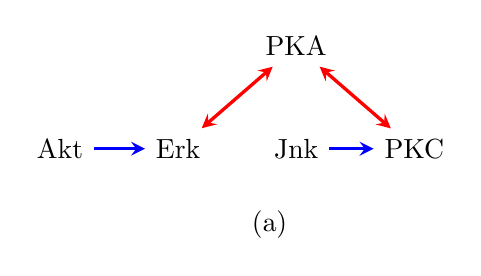
\begin{tikzpicture}[>=stealth, node distance=1.5cm]
		\tikzstyle{format} = [thick, circle, minimum size=1.0mm, inner sep=0pt]
		\tikzstyle{square} = [draw, thick, minimum size=1.0mm, inner sep=3pt]

		\begin{scope}[xshift=0cm]
		\path[->, very thick]
		node[] (akt) {Akt}
		node[right of=akt] (erk) {Erk}
		node[right of=erk] (jnk) {Jnk}
		node[right of=jnk] (pkc) {PKC}
		node[above of=jnk, yshift=-0.2cm] (pka) {PKA}
		node[below right of=erk, xshift=0.1cm, yshift=0.1cm] (label) {(a)}

		(akt) edge[blue] (erk)
		(jnk) edge[blue] (pkc)
		(erk) edge[red, <->] (pka)
		(pka) edge[red, <->] (pkc)
		;
		\end{scope}
		\end{tikzpicture}
	}
\end{center}
In the reweighted $q=\frac{p(\text{Akt, Erk, PKA, Jnk, PKC})}{p(\text{Jnk} \mid \text{Erk, PKA})}$, we have $\text{PKC} \ci_q \text{Akt}$, corresponding to a generalized equality constraint $q(\text{PKC} \mid \text{Akt})=q(\text{PKC})$
}
\vspace{1em}

Remember all constraints for parts a), b), and c) must be between Akt and PKC.

4) Given the above exercise in part 3), argue that the three causal hypotheses of $\text{Erk} \biedge \text{PKA}$,  $\text{PKA} \diedgeright \text{Erk}$, and $\text{Erk} \diedgeright \text{PKA}$ can be distinguished using observed data without the need for a physical lab experiment. In doing so, briefly describe how to conduct a statistical test based on a Verma constraint (you may use the odds ratio as a measure of association) and how this allows us to avoid performing new (potentially expensive or difficult) experiments in the lab. (6 points)

\problemAnswer{
Testing the equality constraints from (a) and (b) is pretty straightforward, we can apply the methods we've used previously in the class. Compute the odds ratio $\odds(\text{Akt},\text{Erk} \mid Z)$ (filling in the appropriate $Z$ as described above), apply bootstrapping to find a 95\% confidence interval, and reject the model if 1 falls outside of the interval. We can also, however, test the Verma constraint with only the data that was already collected using the reweighted distribution $q=\frac{p(\text{Akt, Erk, PKA, Jnk, PKC})}{p(\text{Jnk} \mid \text{Erk, PKA})}$ (note the denominator that we need for reweighting relies only on data that we've measured) and then applying the same odds ratio-based hypothesis testing scheme to test $\text{PKC} \ci_q \text{Akt}$ with this reweighted distribution.
}
\vspace{1em}


\bibliographystyle{apalike}
\bibliography{references}






\end{document}
